\documentclass{gtpart}
\usepackage{amsmath,amssymb,amsthm,stmaryrd}
\usepackage[all]{xy}
\usepackage{tikz}
\usepackage{url}
\usepackage{hyperref}
\usepackage{enumerate}
\usepackage{tensor}
%/home/grad/zyf/TeX/inputs/
\usepackage{mathrsfs}
\usepackage{graphicx}
\usepackage{mathtools}
%\usepackage{amsrefs}
%\usepackage{setspace}
%\doublespacing

\title{The power operation structure on Morava $E$-theory of height 2 at the prime 3}
\author{Yifei Zhu}
\givenname{Yifei}
\surname{Zhu}
\address{Department of Mathematics\\University of Minnesota\\Minneapolis, MN 55455\\USA}
\email{zyf@math.umn.edu}

%\subject{primary}{msc2000}{55P99}
%\subject{secondary}{msc2000}{55Q99}

%\bibliographystyle{gtart}
\parskip 0.7pc
\parindent 0pt

\newtheorem{thm}{Theorem}
\newtheorem{cor}[thm]{Corollary}
\newtheorem{prop}[thm]{Proposition}
\newtheorem{lem}[thm]{Lemma}
\theoremstyle{definition}
\newtheorem{defn}[thm]{Definition}
\theoremstyle{remark}
\newtheorem{rmk}[thm]{Remark}
\newtheorem{exam}[thm]{Example}
\newtheorem{case}[thm]{Case}
\newtheorem{slogan}[thm]{Slogan}
\newtheorem{ques}[thm]{Question}

\def\co{\colon\thinspace}
\newcommand{\mb}[1]{\mathbb{#1}}
\newcommand{\mf}[1]{\mathfrak{#1}}

\newcommand{\NB}[1]{{\bf (NB: #1)}}

\newcommand{\Ext}{\ensuremath{{\rm Ext}}}
\newcommand{\Coext}{\ensuremath{{\rm Coext}}}
\newcommand{\Hom}{\ensuremath{{\rm Hom}}}
\newcommand{\Tor}{\ensuremath{{\rm Tor}}}
\newcommand{\Ind}{\ensuremath{{\rm Ind}}}
\newcommand{\Res}{\ensuremath{{\rm Res}}}
\newcommand{\colim}{\ensuremath{\mathop{\rm colim}}}
\newcommand{\hocolim}{\ensuremath{\mathop{\rm hocolim}}}
\newcommand{\holim}{\ensuremath{\mathop{\rm holim}}}
\newcommand{\overto}{\mathop\rightarrow}
\newcommand{\overfrom}{\mathop\leftarrow}
\newcommand{\into}{\mathop\hookrightarrow}
\newcommand{\onto}{\mathop\twoheadrightarrow}
\newcommand{\longoverto}{\mathop{\longrightarrow}}
\newcommand{\Irr}{\ensuremath{\mathop{\rm Irr}}}
\newcommand{\Rep}{\ensuremath{\mathop{\rm Rep}}}
\newcommand{\Map}{\ensuremath{{\rm Map}}}
\newcommand{\GL}{{\rm GL}}
\newcommand{\Uni}{{\rm U}}
\newcommand{\BU}{{\rm BU}}
\newcommand{\Sp}{{\cal S}p}
\newcommand{\Sym}{{\rm Sym}}
\newcommand{\thh}{{\rm thh}}
\newcommand{\TAF}{{\rm TAF}}
\newcommand{\TAQ}{{\rm TAQ}}
\newcommand{\End}{{\rm End}}
\newcommand{\Aut}{{\rm Aut}}
\newcommand{\As}{{\cal A}s}
\newcommand{\LT}{{\rm LT}}
\newcommand{\Spec}{{\rm Spec\thinspace}}
\newcommand{\Spf}{{\rm Spf}}
\newcommand{\tmf}{{\rm tmf}}
\newcommand{\eo}{{\rm eo}}
\newcommand{\TMF}{{\rm TMF}}
\newcommand{\Ell}{{\cal E}ll}
\newcommand{\Lie}{{\rm Lie}}
\newcommand{\Sh}{{\rm Sh}}
\newcommand{\HF}{{\rm H}{\mb F}}
\newcommand{\cF}{\overline {\mb F}}
\newcommand{\cQ}{\overline {\mb Q}}

\newcommand{\eilm}[1]{\ensuremath{{\mb H} #1}}
\newcommand{\smsh}[1]{\ensuremath{\mathop{\wedge}_{#1}}}
\newcommand{\tens}[1]{\ensuremath{\mathop{\otimes}_{#1}}}
\newcommand{\susp}{\ensuremath{\Sigma}}
\newcommand{\mapset}[3]{\ensuremath{\left[#2,#3\right]_{#1}}}
\newcommand{\form}[2]{\ensuremath{\left\langle#1,#2\right\rangle}}
\newcommand{\bilin}[2]{\ensuremath{\left(#1,#2\right)}}
\newcommand{\comp}[1]{\ensuremath{#1^\wedge}}
\newcommand{\loca}[3]{\ensuremath{L^{#1}_{#2}(#3)}}
\newcommand{\tc}[3]{\ensuremath{\Omega_{#2 / #1}^{#3}}}
\newcommand{\atc}[3]{\ensuremath{\L_{#2 / #1}^{#3}}}

\newcommand{\xym}[1]{
\vskip 0.7pc
\centerline{\xymatrix{#1}}
\vskip 0.7pc
}

\newcommand{\CA}{{\cal A}}
\newcommand{\Mod}{{\rm Mod}}
\newcommand{\Alg}{{\rm Alg}}
\newcommand{\Frob}{{\rm Frob}}
\newcommand{\DF}{{{\rm DefFrob}_\Gamma}}
\newcommand{\Model}{{\rm Model}}
\newcommand{\Gm}{{{\mb G}_m}}
\newcommand*{\longhookrightarrow}{\ensuremath{\lhook\joinrel\relbar\joinrel\rightarrow}}
\newcommand{\cf}{cf.\thinspace}

\newcommand{\DL}{Dyer--Lashof~}
\newcommand{\BF}{{\mb F}}
\newcommand{\BG}{{\mb G}}
\newcommand{\BP}{{\mb P}}
\newcommand{\BZ}{{\mb Z}}
\newcommand{\HC}{\widehat{C}}
\newcommand{\HS}{\widehat{S}}
\newcommand{\TC}{\widetilde{C}}
\newcommand{\TE}{\widetilde{E}}
\newcommand{\Tf}{\widetilde{f}}
\newcommand{\Tw}{\widetilde{w}}
\newcommand{\TP}{\widetilde{\psi}}
\newcommand{\md}{~~{\rm mod}~}
\newcommand{\ad}{{\rm and}}
\newcommand{\A}{\alpha}
\newcommand{\G}{\Gamma}
\newcommand{\g}{\gamma}
\newcommand{\p}{\psi^3}
\newcommand{\CM}{{\mathscr{M}}}
\newcommand{\isog}[1]{Proposition \ref{prop:isog}\thinspace (#1)}


\begin{document}
\begin{abstract}
 We give explicit calculations of the algebraic theory of power operations for a specific Morava $E$-theory spectrum and its $K(1)$-localization.  
 At height 2 for the prime 3, the power operations arise from the universal degree-3 isogeny of elliptic curves associated to the $E$-theory.  
\end{abstract}


\maketitle
\section{Introduction}

The study of cohomology operations has been central to algebraic topology 
since the 1950s, with applications to solving problems such as the non-existence of maps of Hopf invariant one, 
and the maximum number of linearly independent vector fields on spheres.  
Perhaps internally cohomology operations are primarily used to cure the blindness of cohomology theories \cite{blind}, 
that is, to cure their varied degrees of inability to detect the fact that a map of spaces is essential.  

Suppose $E$ is a commutative $S$-algebra, in the sense of \cite{EKMM}, and $A$ is a commutative $E$-algebra.  
We want to capture the properties and underlying structure of the homotopy groups $\pi_* A = A_*$ of $A$, 
by studying operations associated to the cohomology theory that $E$ represents.  

An important family of cohomology operations, called {\em power operations}, is constructed via the extended powers.  
Specifically, consider the functor of {\em the $m$th extended power over $E$} from the category of $E$-modules to the category of commutative $E$-algebras 
\[
 \BP_E^m (-) \coloneqq (-)^{\wedge_E m} / \Sigma_m \co \Mod_E \to \Alg_E 
\]
which sends an $E$-module to its $m$-fold smash product over $E$ modulo the action by the symmetric group on $m$ letters.  
The $\BP_E^m (-)$'s assemble together to give the {\em free commutative $E$-algebra} functor 
\[
 \BP_E (-) \coloneqq \bigvee_{m \geq 0} \BP_E^m (-) \co \Mod_E \to \Alg_E.  
\]
These functors descend to homotopy categories.  
In particular, each $\A \in \pi_{d+i}~\BP_E^m (\Sigma^d E)$ gives rise to a power operation 
\[
 Q_\A \co A_d \to A_{d+i} 
\]
(\cf \cite[Sections I.2 and IX.1]{H_infty} and \cite[Section 3]{cong}).  

Under the action of power operations, $A_*$ is an algebra over some operad on $E_*$-modules involving the structure of $E_* B\Sigma_m$ for all $m$.  
This operad is traditionally called a {\em \DL algebra}, or more precisely, 
a \DL {\em theory} as the {\em algebraic theory} of power operations acting on the homotopy groups of commutative $E$-algebras 
(\cf \cite[Chapters III, VIII, and IX]{H_infty} and \cite[Section 9]{lpo}).  

A specific case is when $E$ represents a Morava $E$-theory of height $n$, and $A$ is $K(n)$-local.  
Morava $E$-theory spectra are of crucial importance in modern stable homotopy theory, 
particularly in the work of Ando, Hopkins, and Strickland \cite{cube}.  
Much of the $K(n)$-local $E$-\DL theory has been worked out by those authors (\cf \cite[1.5]{cong} for a description of the history).  
In \cite{cong} Rezk gives a unified treatment of this \DL theory.  
He works out a congruence criterion that must hold in an algebra over the \DL theory (\cite[Theorem A]{cong}).  
This enables one to study the \DL {\em theory}, which models all the algebraic structure naturally adhering to $A_*$, 
by working with a certain associative ring $\G$ as the \DL {\em algebra}.  
Moreover, Rezk provides a geometric description of this congruence criterion, 
in terms of sheaves on the moduli problem of deformations of formal groups and Frobenius isogenies (\cf \cite[Theorem B]{cong}).  
This connects the structure of $\G$ to the geometry underlying $E$, 
moving one step forward from a workable object $\G$ to things that are computable.  
Based on these, in a companion paper \cite{h2p2}, 
Rezk gives explicit calculations of the \DL theory for a specific Morava $E$-theory of height $n = 2$ at the prime 2.  

The purpose of this paper is to make available calculations analogous to some of the results in \cite{h2p2}, at the prime 3, 
together with calculations of the corresponding $K(1)$-local power operations.  


\subsection{Outline of the paper}

As in \cite{h2p2}, the computation of power operations in this paper follows the approach of \cite{steenrod}: 
one first defines a total power operation, 
and then uses the computation of the cohomology of the classifying space of the symmetric group $\Sigma_m$ to obtain individual power operations.  
These two steps are carried out in Sections \ref{sec:total} and \ref{sec:individual} respectively.  

In Section \ref{sec:total}, by doing calculations with elliptic curves associated to our Morava $E$-theory $E$, 
we give formulas of the total power operation $\p$ on $E_0$ and the ring $S_3$ which parametrizes the corresponding moduli problem.  

In Section \ref{sec:individual}, based on calculations of $E^* B\Sigma_m$ in \cite{Str98} as reflected in the formula of $S_3$, 
we define individual power operations, and derive the relations they satisfy.  
Thus in view of the general structures studied in \cite{cong}, 
we get an explicit description of the \DL algebra $\G$ for $K(2)$-local commutative $E$-algebras.  

In Section \ref{sec:K(1)}, we describe the relationship between the total power operation $\p$, at height 2, and the corresponding $K(1)$-local power operation.  
We then derive formulas of the latter from the calculations in Section \ref{sec:total}.  

\begin{rmk}
\label{rmk:parameter}
 The ring $S_3$ turns out to be an algebra on one generator over the base ring where our elliptic curve is defined 
 (\cf \isog{i}).  This generator appears as a parameter in the formulas of the total power operation $\p$, 
 and is responsible for how the individual power operations are defined and how their formulas look.  
 Different choices of this parameter result in different bases of the \DL algebra $\G$.  
 The parameter in this paper will be derived differently from the one used in \cite{h2p2}.  
 It comes from the relative cotangent space of the elliptic curve at the identity (\cf \isog{iv}, Corollary \ref{cor:A'}, and Remark \ref{rmk:A'}).  
 This choice of parameter is important for writing down Adem relations in Proposition \ref{prop:Q}\thinspace (iv), 
 and it fits naturally into the treatment of gradings in \cite{cong} (\cf Example \ref{ex:omega} and Theorem \ref{thm:gamma}).  

 We should point out that our choice is by no means canonical.  
 We do not know yet, as part of the structure of the \DL algebra, 
 if there is a canonical basis which is both geometrically interesting and computationally convenient.  
 Somewhat surprisingly, although it appears to come from different considerations, 
 our choice has an analog at the prime 2 which coincides with the parameter used in \cite{h2p2} (\cf Remarks \ref{rmk:A} and \ref{rmk:AA'}).  
 The calculations follow a recipe in hope of generalizing to other Morava $E$-theories at height 2; 
 we hope to address these matters and recognize more of the general patterns based on further computational evidence.  
\end{rmk}


\subsection{Acknowledgements}

I thank Charles Rezk for his encouragement on this work, and for his observation in a correspondence which led to Proposition \ref{prop:frob^2} and Corollary \ref{cor:A'}.  

I thank Kyle Ormsby for directing me to \cite{kohel}.  Remark \ref{rmk:velu} is out of his suggestion.  

I thank Tyler Lawson for the sustained support from him I received as a student.  


\subsection{Conventions}

Let $p$ be a prime, $q$ a power of $p$, and $n$ a positive integer.  We use the symbols 
\[
 \BF_q,~~\cF_q,~~\BZ_q,~~\ad~~\BZ/n 
\]
to denote a field with $q$ elements, an algebraic closure of $\BF_q$, the ring of $p$-typical Witt vectors over $\BF_q$, 
and the additive group of integers modulo $n$, respectively.  

If $R$ is a ring, then $R\llbracket x \rrbracket$ denotes the ring of formal power series over $R$ in the variable $x$.  
If $I \subset R$ is an ideal, then $R_I^\wedge$ denotes the completion of $R$ with respect to $I$.  

If $E$ is an elliptic curve and $m$ is an integer, then $[m]$ denotes the multiplication-by-$m$ map on $E$, and $E[m]$ denotes the $m$-torsion subgroup of $E$.  

All formal groups mentioned in this paper will be commutative and one-dimensional.  

The terminology for describing the structure of the \DL theory will follow \cite{cong} and \cite{h2p2}; 
some of the notions there are taken in turn from \cite{BW} and \cite{V}.  


\section{Total power operations}
\label{sec:total}

\subsection{An elliptic curve and the corresponding Morava $E$-theory spectrum}

The universal generalized elliptic curve $C$ with a choice of 4-torsion point has equation 
\[
 Y^2 Z + a X Y Z + a c Y Z^2 = X^3 + c X^2 Z 
\]
over the graded ring $\BZ [1/4] [a,c]$ with $|a| = 1$ and $|c| = 2$.  
This equation is computed from a general affine Weierstrass equation in $xy$-coordinates, 
by requiring that the chosen point $P$ of $C$ be $(0,0)$, $2P$ be on the $x$-axis, and $4P$ be the identity at the infinity (\cf \cite[4(4.6a)]{ec}).  

In the affine coordinate chart $c = 1$ of the moduli stack $\CM \big(\G_1(4)\big)$, 
$C$ is given by the Weierstrass equation 
\begin{equation}
\label{Cxy}
 y^2 + a x y + a y = x^3 + x^2 
\end{equation}
over the ring $\BZ [1/4] [a]$, and the discriminant of $C$ is $\Delta = a^2 (a + 4) (a - 4)$.  
Let 
\begin{equation}
\label{S}
 S = \BZ [1/4] [a, \Delta^{-1}] 
\end{equation}
over which $C$ is nonsingular.  
Over a finite field of characteristic 3, this nonsingular elliptic curve is supersingular precisely when the quantity 
\begin{equation}
\label{h}
 h \coloneqq a^2 + 4 
\end{equation}
vanishes (\cf \cite[V.4.1a]{AEC}), and its minimal field of definition is then $\BF_9$.  
Moreover the supersingular locus in this coordinate chart consists of a single closed point, as $(3,h)$ is a maximal ideal of $S$.  

We next write 
\[
 \HS = \BZ_9 \llbracket h \rrbracket.  
\]
Let $i$ be an element generating $\BZ_9$ over $\BZ_3$ with $i^2 = -1$.  
Since $h = a^2 + 4$, we have 
\[
 a \equiv i \md (3,h) \qquad \ad \qquad \Delta \equiv -1 \md (3,h), 
\]
where $(3,h)$ is the maximal ideal of the complete local ring $\HS = \BZ_9 \llbracket h \rrbracket$.  
Then by Hensel's lemma, both $a$ and $\Delta$ lie in $\HS$, and both are invertible.  
Thus $\HS$ is the completion of $S$ with respect to $(3,h)$.  

Let $\HC$ be the formal completion of $C$ at the identity; it is a formal group over $\HS$.  
Its reduction to $\BF_9 = \HS / (3,h)$ is a formal group $\BG$ of height 2.  
By Serre--Tate theory, 3-adically the deformation theory of an elliptic curve is equivalent to the deformation theory of its 3-divisible group, 
and thus $\HC$ is the universal deformation of $\BG$.  
Let $E$ be the commutative $S$-algebra which represents the Morava $E$-theory associated to $\BG$.  Then 
\[
 E_* \cong \BZ_9 \llbracket h \rrbracket [u^{\pm 1}] 
\]
with $|u| = 2$, and $u$ corresponds to a local uniformizer at the identity of $C$.  


\subsection{The 3-torsion points on the elliptic curve}

To study $C$ in the formal neighborhood of the identity, it is convenient to make a change of variables.  
Let 
\[
 u = \frac{x}{y} \quad \ad \quad v = \frac{1}{y}, \qquad {\rm so} \qquad x = \frac{u}{v} \quad \ad \quad y = \frac{1}{v}.  
\]
The identity $O$ of $C$ is then $(u,v) = (0,0)$, with $u$ a local uniformizer at $O$.  
The equation \eqref{Cxy} of $C$ becomes 
\begin{equation}
\label{Cuv}
 v + a u v + a v^2 = u^3 + u^2 v.  
\end{equation}

\begin{prop}
\label{prop:tors}
 On the elliptic curve $C$ over $S$, the $uv$-coordinates $(d,e)$ of any nonzero 3-torsion point satisfy the identities 
 \begin{equation}
 \label{f}
  f(d) = 0, 
 \end{equation}
 and 
 \begin{equation}
 \label{g}
  e = g(d), 
 \end{equation}
 where $f, g \in S[u]$ are given by 
 \begin{equation*}
 \begin{split}
  f(u) = & ~ u^8 + 3 a u^7 + 3 a^2 u^6 + (a^3 + 7 a) u^5 + (6 a^2 - 6) u^4 + 9 a u^3 + (-a^2 + 8) u^2 \\
         & - 3 a u - 3, \\
  g(u) = & -\frac{1}{a (a + 4) (a - 4)} \big(a u^7 + (3 a^2 - 2) u^6 + (3 a^3 - 6 a) u^5 + (a^4 + a^2 + 2) u^4 \\
         & + (4 a^3 - 15 a) u^3 + 18 u^2 - 12 a u - 18\big).  
 \end{split}
 \end{equation*}
\end{prop}
\begin{proof}
 \footnote{See Appendix \ref{apx:tors} for formulas of the polynomials $\Tf$, $Q_1$, $R_1$, $Q_2$, $R_2$, $K$, $L$, $M$, and $N$ that appear below.  }
 Given the elliptic curve $C$ with equation \eqref{Cxy}, a nonzero point $Q$ on $C$ is a 3-torsion point if and only if the division polynomial 
 \begin{equation}
 \label{divpoly}
  \psi_3 (x) \coloneqq 3 x^4 + (a^2 + 4) x^3 + 3 a^2 x^2 + 3 a^2 x + a^2 
 \end{equation}
 vanishes at $Q$ (\cf \cite[Exercise 3.7f]{AEC}).  Substituting $x$ by $u/v$ and clearing the denominators, we have a homogeneous polynomial in $u$ and $v$ 
 \[
  \TP_3(u,v) \coloneqq 3 u^4 + (a^2 + 4) u^3 v + 3 a^2 u^2 v^2 + 3 a^2 u v^3 + a^2 v^4.  
 \]
 As $Q = (d,e)$ in $uv$-coordinates, we then have $\TP_3(d,e) = 0$.  

 To get the polynomial $f$, we rewrite the equation \eqref{Cuv} of $C$ as a quadratic equation in $v$ 
 \begin{equation}
 \label{quadratic}
  a v^2 + (-u^2 + a u + 1) v - u^3 = 0, 
 \end{equation}
 where the leading coefficient $a$ is invertible in $S = \BZ [1/4] [a, \Delta^{-1}]$ as $\Delta = a^2 (a + 4) (a - 4)$.  
 Define 
 \begin{equation}
 \label{Tfdef}
  \Tf(u) = \TP_3(u,v) \TP_3(u,\bar{v}), 
 \end{equation}
 where $v$ and $\bar{v}$ are formally the conjugate roots of \eqref{quadratic} 
 so that we compute $\Tf$ in terms of $u$ by substituting $v + \bar{v}$ as $(u^2 - a u - 1) / a$, and $v \bar{v}$ as $-u^3 / a$.  
 We then factor $\Tf$ over $S$ as 
 \begin{equation}
 \label{Tffactor}
  \Tf(u) = -\frac{u^4 f(u)}{a^2}, 
 \end{equation}
 where $f$ is the stated degree-8 polynomial.  
 We check that $f$ is irreducible by applying Eisenstein's criterion to the prime ideal $(3,h)$ of the unique factorization domain $S$.  

 We have $\Tf(d) = 0$ by \eqref{Tfdef}; to see $f(d) = 0$, consider the closed subscheme $C[3]^\times \subset C$ of points of exact order 3.  
 It is finite over $S$ of rank 8 by \cite[Theorem 2.3.1]{KM}.  
 By the Cayley--Hamilton theorem, as a global section of $C[3]^\times$, $u$ locally satisfies a degree-8 equation, 
 and this equation then locally defines the rank-8 scheme $C[3]^\times$.  
 Since $C[3]^\times$ does not contain the identity, it is affine, and thus it is globally defined by a degree-8 equation in $u$.  
 In view of $\Tf(d) = 0$ and \eqref{Tffactor}, we then determine this equation and get the first stated identity \eqref{f}.  

 To get the polynomial $g$, we note that both the quartic polynomial 
 \[
  A(v) \coloneqq \TP_3(d,v) 
 \]
 and the quadratic polynomial 
 \[
  B(v) \coloneqq a v^2 + (-d^2 + a d + 1) v - d^3 
 \]
 vanish at $e$, and thus so does their greatest common divisor (gcd).  Using the Euclidean algorithm, we have 
 \begin{equation*}
 \begin{split}
  A(v) = & ~ Q_1(v) B(v) + R_1(v), \\
  B(v) = & ~ Q_2(v) R_1(v) + R_2, 
 \end{split}
 \end{equation*}
 where 
 \[
  R_1(v) = K(d) v + L(d) 
 \]
 for some polynomials $K$ and $L$, and $R_2 = 0$ in view of \eqref{f}.  Thus $R_1(v)$ is the gcd of $A(v)$ and $B(v)$, and hence 
 \[
  K(d) e + L(d) = R_1(e) = 0.  
 \]
 To write $e$ in terms of $d$ from the above identity, we apply the Euclidean algorithm to the polynomials $f$ and $K$.  
 Their gcd turns out to be 1, and thus there are polynomials $M$ and $N$ such that 
 \[
  M(u) f(u) + N(u) K(u) = 1.  
 \]
 By \eqref{f} we then have $N(d) K(d) = 1$, and thus 
 \[
  e = -N(d) L(d) = g(d), 
 \]
 where $g$ is as stated.  
\end{proof}

\begin{rmk}
\label{rmk:dmod3}
 We have 
 \[
  f(u) \equiv u^2 (u^6 + a h u^3 - h) \md 3.  
 \]
 The two roots (counted with multiplicity) of $f(u)$ which reduce to zero modulo 3 correspond to 
 the two nonzero points in the unique order-3 subgroup of $C$ in the formal neighborhood of the identity.  
\end{rmk}


\subsection{The universal degree-3 isogeny and the corresponding total power operation}

\begin{prop}
\label{prop:isog}
 \mbox{}
 \begin{enumerate}[(i)]
  \item The universal degree-3 isogeny $\psi$ with source $C$ is defined over the ring 
  \[
   S_3 \coloneqq S[\A] \big/ \big( w(\A) \big) 
  \]
  where 
  \[
   w(\A) = \A^4 - 6 \A^2 + (a^2 - 8) \A - 3, 
  \]
  and has target the elliptic curve 
  \[
   C' \co v + r(a) u v + r(a) v^2 = u^3 + u^2 v, 
  \]
  where 
  \[
   r(a) = a^3 + (\A^3 - 6 \A - 12) a - 4 (\A + 1)^2 (\A - 3) a^{-1}.  
  \]

  \item The isogeny $\psi$ restricts to the supersingular locus as the third-power Frobenius isogeny.  

  \item The kernel of $\psi$ is generated by a 3-torsion point $Q$ with coordinates $(d,e)$ satisfying 
  \begin{equation}
  \label{A}
  \begin{split}
   \A = & -\frac{1}{(a + 4) (a - 4)} \big(a d^7 + (3 a^2 - 2) d^6 + (3 a^3 - 6 a) d^5 + (a^4 + a^2 + 2) d^4 \\
        & + (4 a^3 - 15 a) d^3 + (a^2 + 2) d^2 - 12 a d -18\big) \\
      = & ~ a e - d^2.  
  \end{split}
  \end{equation}

  \item The induced map $\psi^*$ on relative cotangent spaces at the identity sends $du$ to $\A du$.  
 \end{enumerate}
\end{prop}
\begin{proof}
 \footnote{See Appendix \ref{apx:isog} for the formula of the power series expansion of $v$, 
 and details of the calculations involving the group law on $C$ that appear below.  }
 Let $P = (u,v)$ be a general point on $C$, and $Q = (d,e)$ be a nonzero 3-torsion point.  
 Rewriting the equation \eqref{Cuv} of $C$ as 
 \[
  v = u^3 + u^2 v - a u v - a v^2, 
 \]
 we express $v$ in terms of a formal power series in $u$ by recursive substitution.  
 For the purpose of our calculations, we take this power series up to $u^9$ as an expression of $v$, 
 and write $e = g(d)$ as in \eqref{g}.  

 We define functions $u'$ and $v'$ by 
 \begin{equation}
 \label{u'v'def}
 \begin{split}
  u' = & ~ u(P) \cdot u(P-Q) \cdot u(P+Q), \\
  v' = & ~ v(P) \cdot v(P-Q) \cdot v(P+Q), 
 \end{split}
 \end{equation}
 where $u(-)$ and $v(-)$ denote the $u$-coordinate and $v$-coordinate of a point respectively.  
 By computing the group law on $C$, we express $u'$ and $v'$ in terms of formal power series in $u$: 
 \begin{equation}
 \label{u'v'formula}
 \begin{split}
  u' = & ~ \A u + \text{higher degree terms}, \\
  v' = & ~ \beta u^3 + \text{higher degree terms}, 
 \end{split}
 \end{equation}
 where the coefficients ($\A$, $\beta$, etc.) involve $a$ and $d$.  
 In particular, in view of \eqref{f}, we compute that $\A$ satisfies $w(\A) = 0$, where $w$ is as stated in (i).  

 Now define the isogeny $\psi \co C \to C'$ by 
 \begin{equation}
 \label{psi}
  u\big(\psi(P)\big) = u' \qquad \ad \qquad v\big(\psi(P)\big) = \frac{\A^3}{\beta} \cdot v', 
 \end{equation}
 where we introduce the normalizing factor $\A^3 / \beta$ so that the equation of $C'$ will be in the form of \eqref{Cuv}.  
 The kernel of $\psi$ is precisely the order-3 subgroup generated by $Q$.  
 Using \eqref{u'v'formula}, we then determine the coefficients of a general Weierstrass equation that $u\big(\psi(P)\big)$ and $v\big(\psi(P)\big)$ satisfy.  
 This is the stated equation of $C'$ in (i).  

 We next check the statement of (ii).  
 Recall that the ideal $(3,h)$ of $S$ corresponds to the supersingular locus $\BF_9 = S / (3,h)$.  
 Since there is no nonzero 3-torsion point over the supersingular locus, we have 
 \[
  d \equiv e \equiv 0 \md (3,h).  
 \]
 Using this congruence and the formulas \eqref{P-Q} \eqref{P+Q} of $u(P-Q)$ and $u(P+Q)$ in Appendix \ref{apx:isog}, we compute that 
 \begin{equation}
 \label{deffrob}
  u\big(\psi(P)\big) = u(P) \cdot u(P-Q) \cdot u(P+Q) \equiv u^3 \md (3,h).  
 \end{equation}
 As the $u$-coordinate is a local uniformizer at the identity, $\psi$ restricts to the supersingular locus as the third-power Frobenius isogeny.  

 For the remaining statements of the proposition, 
 in \eqref{A}, the first identity is computed in \eqref{u'v'formula}; 
 we then check the second identity by comparing the previous one with the formula of $g$ in Proposition \ref{prop:tors}.  
 The statement of (iv) follows by definition of $\A$ in \eqref{u'v'formula}.  
\end{proof}

\begin{rmk}
 In view of \isog{ii}, the formal completion of $\psi \co C \to C'$ at the identity of $C$ 
 is a {\em deformation of the third-power Frobenius isogeny}, in the sense of \cite[11.3]{cong}.  
 When it is clear from the context, we will simply call $\psi$ itself a deformation of the third-power Frobenius isogeny.  
\end{rmk}

\begin{rmk}
\label{rmk:A}
 The analog of $\A$ at the prime 2 coincides with $d$, studied in \cite[Section 3]{h2p2}, 
 which is the $u$-coordinate of a nonzero 2-torsion point on the universal elliptic curve with a choice of 3-torsion point 
 (\cf \cite[Proposition 3.2]{tmf3}).  
\end{rmk}

In [Str98] Strickland shows that 
\[
 \HS_3 \cong E^0 B\Sigma_3 / I, 
\]
where 
\[
 \HS_3 \coloneqq \big( S_3 \big)_{(3,h)}^\wedge \cong \HS \otimes_S S_3, 
\]
and
\begin{equation}
\label{transfer}
 I \coloneqq \bigoplus_{0<i<3} {\rm image} \big( E^0 B(\Sigma_i \times \Sigma_{3-i}) \xrightarrow{\rm transfer} E^0 B\Sigma_3 \big) 
\end{equation}
is the {\em transfer ideal}.  
In view of this and the construction of {\em total power operations} for Morava $E$-theories in \cite[3.23]{cong}, we have the following corollary.  
\begin{cor}
\label{cor:psi3}
 The total power operation 
 \[
  \p \co E^0 \to E^0 B\Sigma_3 / I \cong E^0 [\A] \big/ \big( w(\A) \big) 
 \]
 is given by 
 \begin{equation*}
 \begin{split}
  \p(h) = & ~ h^3 + (\A^3 - 6 \A - 36) h^2 + 3 (-8 \A^3 + \A^2 + 48 \A + 130) h \\
          & + 4 (30 \A^3 - 9 \A^2 - 178 \A - 303), \\
  \p(a) = & ~ a^3 + (\A^3 - 6 \A - 12) a - 4 (\A + 1)^2 (\A - 3) a^{-1}, 
 \end{split}
 \end{equation*}
 where 
 \begin{equation}
 \label{Amod3}
  \A \equiv 0 \md 3, 
 \end{equation}
 so that 
 \[
  \p(h) \equiv h^3 \md 3 \qquad \ad \qquad \p(a) \equiv a^3 \md 3.  
 \]
\end{cor}
\begin{proof}
 By \cite[Theorem B]{cong}, there is a correspondence between the universal degree-3 isogeny $\psi$ with source $C$, which is a deformation of Frobenius, 
 and the total power operation $\p$ with domain $E^0$.  In particular $\p(a)$ is given by the polynomial $r(a)$ in \isog{i}.  
 As $\p$ is a ring homomorphism, we then get the formula of $\p(h) = \p(a^2 + 4)$.  

 The congruence \eqref{Amod3} follows from Remark \ref{rmk:dmod3} and \eqref{A}.  
\end{proof}

\begin{rmk}
\label{rmk:velu}
 As mentioned in Remark \ref{rmk:parameter}, there are different possible choices of the parameter in the total power operation $\p$.  
 Here we record one which is obtained in $xy$-coordinates following V\'elu's formulas \cite{velu} as presented in \cite[Section 2.4]{kohel}.  
 For computing the formulas of $\p$, this choice of parameter is considerably more convenient than using $\A$, 
 as the group law on the elliptic curve is encoded in V\'elu's formulas.  

 We continue with the notations in Proposition \ref{prop:isog}.  
 Let $s$ be the $x$-coordinate of the 3-torsion point $Q$.  
 As in \eqref{divpoly}, it satisfies 
 \begin{equation}
 \label{Tw}
  \Tw(s) \coloneqq 3 s^4 + (a^2 + 4) s^3 + 3 a^2 s^2 + 3 a^2 s + a^2 = 0.  
 \end{equation}
 We then have 
 \[
  S_3 = S[s] \big/ \big( \Tw(s) \big), 
 \]
 and 
 \[
  C' \co y^2 + r(a) x y + r(a) y = x^3 + x^2, 
 \]
 where 
 \begin{equation*}
 \begin{split}
  r(a) = & ~ (s + 1) (4 s + 5) a + 4 s^2 (3 s + 4) a^{-1} \\
       = & ~ (s^{-1} + 1)^3 a^3 - (4 s^{-1} + 3) a.  
 \end{split}
 \end{equation*}
 Thus, as in Corollary \ref{cor:psi3}, correspondingly we get formulas 
 \begin{equation*}
 \begin{split}
  \p(h) = & ~ (s^{-1} + 1)^3 h^3 - (22 s^{-3} + 69 s^{-2} + 75 s^{-1} + 27) h^2 \\
          & + (128 s^{-3} + 424 s^{-2} + 512 s^{-1} + 201) h \\
          & - 16 (14 s^{-3} + 49 s^{-2} + 65 s^{-1} + 27), \\
  \p(a) = & ~ (s^{-1} + 1)^3 a^3 - (4 s^{-1} + 3) a, 
 \end{split}
 \end{equation*}
 where 
 \begin{equation}
 \label{tmod3}
  s^{-1} \equiv 0 \md 3.  
 \end{equation}
 Since $s = d / e$, and in view of \eqref{g} and \eqref{A}, we have a relation 
 \[
  \A (s + 1) = -1 
 \]
 in the ring $S[d] \big/ \big( f(d) \big)$.  
 We then check that the formulas of $\p$ above and those in Corollary \ref{cor:psi3} agree via this relation.  
 See Appendix \ref{apx:velu} for details of the calculations.  
\end{rmk}


\section{Individual power operations}
\label{sec:individual}

\subsection{Composition of deformations of Frobenius isogenies}

Recall from Proposition \ref{prop:isog} that we have the universal degree-3 isogeny $\psi \co C \to C' = C/G$, where $G$ is an order-3 subgroup of $C$; 
in particular, $\psi$ is a deformation of the third-power Frobenius isogeny over the supersingular locus.  
We want to construct a similar isogeny $\psi'$ with source $C'$ 
so that the composite $\psi' \circ \psi$ will correspond to a composite of total power operations via \cite[Theorem B]{cong}.  

Let $G' = C[3]/G$ which is an order-3 subgroup of $C'$ 
(if $G$ is the unique order-3 subgroup of $C$ in the formal neighborhood of the identity, $G'$ is the unique subgroup of $C'$ with the same property).  
We then define $\psi' \co C' \to C'/G'$ using a nonzero point in $G'$ as in \eqref{u'v'def} and \eqref{psi}.  
As the equation of $C'$ in \isog{i} is in the form of \eqref{Cuv}, 
we check as in \eqref{deffrob} that $\psi'$ is also a deformation of the third-power Frobenius isogeny.  

\begin{prop}
\label{prop:frob^2}
 The following diagram of elliptic curves over $S_3$ commutes: 
 \begin{equation}
 \label{frob^2}
  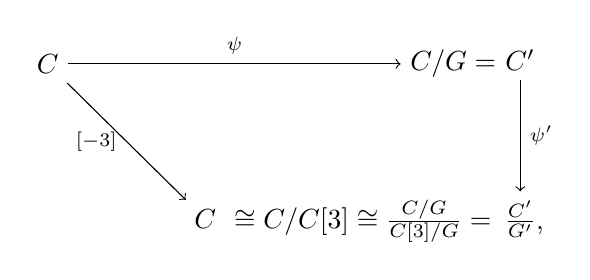
\begin{tikzpicture}[baseline=(current bounding box.center)]
          \node (LT) at (0, 2) {$C$}; 
          \node (MT) at (5.15, 2) {$C/G = $}; 
          \node (RT) at (6, 2.05) {$C'$}; 
          \node (LB) at (2, 0.03) {$C$}; 
          \node (MB) at (4, 0) {$ \cong C/C[3] \cong \frac{C/G}{C[3]/G} = $}; 
          \node (RB) at (6, 0.025) {$\frac{C'}{G'}$}; 
          \node at (6.25, -0.125) {,}; 
          \draw [->] (LT) -- node [above] {$\scriptstyle \psi$} (MT); 
          \draw [->] (LT) -- node [left] {$\scriptstyle [-3]$} (LB); 
          \draw [->] (RT) -- node [right] {$\scriptstyle \psi'$} (RB); 
  \end{tikzpicture}
 \end{equation}
 where the isomorphisms in the bottom row are the canonical ones.  
\end{prop}
\begin{proof}
 In view of \eqref{h}, over the supersingular locus $\BF_9$ the equation of $C$ is 
 \[
  y^2 + i x y + i y = x^3 + x^2, 
 \]
 where $i$ is an element generating $\BF_9$ over $\BF_3$ with $i^2 = -1$.  
 Let $\psi_0$ and $\psi'_0$ be the restrictions of $\psi$ and $\psi'$ over $\BF_9$ respectively.  
 As they are the third-power Frobenius isogenies by \isog{ii}, we have 
 \[
  \psi_0 \co C \to C' \qquad \ad \qquad \psi'_0 \co C' \to C, 
 \]
 where $C'$ has equation 
 \[
  y^2 - i x y - i y = x^3 + x^2.  
 \]
 Thus the composite $\psi'_0 \circ \psi_0$ is the ninth-power Frobenius endomorphism of $C$ over $\BF_9$.  
 We claim that this composite coincides with the endomorphism $[-3]$.  

 Consider the elliptic curve 
 \[
  \TC \co y^2 = x^3 + x - 1 
 \]
 over $\BF_3$.  It is supersingular by \cite[V.4.1a]{AEC}, and over $\BF_9$ it is isomorphic to $C$ via 
 \[
  x \mapsto x, \qquad y \mapsto y - i x - i.  
 \]
 Let $\TP_0$ be the third-power Frobenius endomorphism of $\TC$.  
 By \cite[Theorem 2.6.3]{KM}, in the endomorphism ring of $\TC$, $\TP_0$ is a root of the $\BZ$-polynomial 
 \begin{equation}
 \label{charpoly}
  X^2 - {\rm trace}(\TP_0) \cdot X + 3, 
 \end{equation}
 where $\big( {\rm trace}(\TP_0) \big)^2 \leq 4 \cdot 3$.  
 Moreover by \cite[Exercise 5.10a]{AEC}, since $\TC$ is supersingular, ${\rm trace}(\TP_0) \equiv 0 \md 3$.  
 Thus ${\rm trace}(\TP_0) = 0$, 3, or $-3$.  
 We exclude the latter two possibilities by checking the action of $\TP_0$ at the 2-torsion point $(-1,0)$.  
 It then follows from \eqref{charpoly} that the ninth-power Frobenius endomorphism $\TP_0 \circ \TP_0$ agrees with $[-3]$ on $\TC$ over $\BF_3$.  
 Since $C$ and $\TC$ are isomorphic over $\BF_9$, the composite $\psi'_0 \circ \psi_0$, 
 which is the ninth-power Frobenius endomorphism on $C$, then coincides with $[-3]$ as claimed.  

 It remains to show that $\psi'_0 \circ \psi_0 = [-3]$ over $\BF_9$ lifts to 
 \[
  \psi' \circ \psi = [-3] \co C \to C'/G' 
 \]
 over $S_3$, where by abuse of notation $[-3]$ denotes the endomorphism $[-3]$ of $C$ composed with the canonical isomorphisms from $C$ to $C'/G'$.  
 \footnote{Besides the one given below, there is an argument which works in greater generality, 
 under the assumption that $\psi' \circ \psi$ and $[-3]$ are morphisms of abelian schemes over a connected base scheme 
 (\cf \cite[Proposition 6.1 and Corollary 6.2]{GIT}).  }

 By \cite[Theorem 2.3.1]{KM}, since 4 is invertible in $S_3$ (\cf \isog{i} and \eqref{S}), 
 both $C[4]$ and $(C'/G')[4]$ are finite \'etale over $S_3$.  
 Consider the commutative diagram 
 \begin{center}
 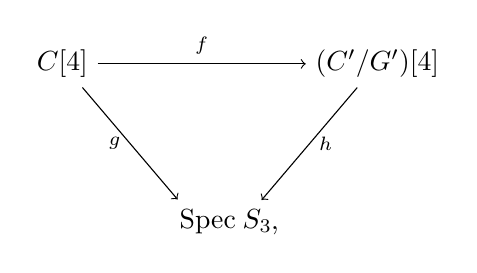
\begin{tikzpicture}
         \node (LT) at (0, 2) {$C[4]$}; 
         \node (RT) at (4, 2) {$(C'/G')[4]$}; 
         \node (MB1) at (1.7, 0) {$~~~\Spec$}; 
         \node (MB2) at (2.3, 0) {$~~~S_3$}; 
         \node at (2.7, -0.125) {,}; 
         \draw [->] (LT) -- node [above] {$\scriptstyle f$} (RT); 
         \draw [->] (LT) -- node [left] {$\scriptstyle g$} (MB1); 
         \draw [->] (RT) -- node [right] {$\scriptstyle h$} (MB2); 
 \end{tikzpicture}
 \end{center}
 where $f$ denotes the restriction of $\psi' \circ \psi - [-3]$ to $C[4]$, and $g$ and $h$ are the structure morphisms.  
 Since $h$ is finite \'etale, it is separated (\cf \cite[Appendix D]{GW}) and unramified, 
 and thus the zero-section $O$ of $(C'/G')[4]$ is closed and open 
 by \cite[Proposition \href{http://math.columbia.edu/algebraic_geometry/stacks-git/locate.php?tag=024T}{024T}]{stacks-project}.  
 Since $g$ is finite \'etale, it is closed and open (\cf \cite[Appendix D]{GW}), 
 and thus $Z \coloneqq g \big( C[4] \setminus f^{-1}(O) \big)$ is closed and open in $\Spec S_3$.  
 Since $\Spec S_3$ is connected and $Z$ does not contain the supersingular locus, $Z$ is empty.  
 Thus $\psi' \circ \psi$ and $[-3]$ agree on $C[4]$.  
 Similarly, they agree on $C[4^k]$ for all positive integers $k$.  

 Now let $F$ denote $\psi' \circ \psi - [-3]$ defined on the entire $C$.  
 Let $s \in \Spec S_3$, and $(-)_s$ be the fiber over $s$ of the structure morphism.  
 By faithfully flat descent, we may assume that $s$ is a geometric point.  
 Since $(C'/G')_s$ is separated over $S_3$, 
 its zero-section $O$ is closed by \cite[Proposition \href{http://math.columbia.edu/algebraic_geometry/stacks-git/locate.php?tag=024T}{024T}]{stacks-project}, 
 and thus $F_s^{-1}(O)$ is closed.  
 Since $C_s$ is an irreducible one-dimensional noetherian scheme, 
 the closed subsets are $C_s$ itself and finite sets of closed points (\cf \cite[Corollary 15.3]{GW}).  
 We have seen that $F_s^{-1}(O)$ contains $C_s[4^k]$ for all $k$.  
 By \cite[Theorem 2.3.1]{KM}, $\{ C_s[4^k] \}_{k \geq 1}$ is a strictly increasing sequence of subschemes of $C_s$ (with respect to inclusion).  
 In particular it is not contained in any closed subset other than $C_s$ itself.  
 Hence $F_s^{-1}(O) = C_s$.  
\end{proof}

Analogous to \isog{iv}, let $\A'$ be the element in $S_3$ such that $(\psi')^*$ sends $du$ to $\A' du$.  

\begin{cor}
\label{cor:A'}
 The following relations hold in $S_3$: 
 \[
  \A \A' + 3 = 0, 
 \]
 and 
 \[
  \A' = -\A^3 + 6 \A + (-a^2 + 8).  
 \]
\end{cor}
\begin{proof}
 The isogenies in \eqref{frob^2} induce maps on relative cotangent spaces at the identity.  
 By \isog{iv} we then have a commutative diagram 
 \begin{center}
 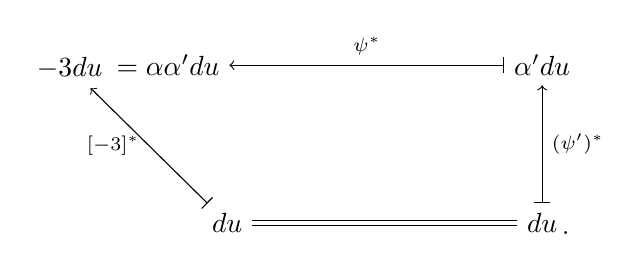
\begin{tikzpicture}
         \node (LT) at (0, 1.97) {$-3 du$}; 
         \node (MT) at (1.25, 2) {$= \A \A' du$}; 
         \node (RT) at (6, 2) {$\A' du$}; 
         \node (LB) at (2, 0) {$du$}; 
         \node (RB) at (6, 0) {$du$}; 
         \node at (6.3, -0.125) {.}; 
         \draw [|->] (RT) -- node [above] {$\scriptstyle \psi^*$} (MT); 
         \draw [|->] (LB) -- node [left] {$\scriptstyle [-3]^*$} (LT); 
         \draw [|->] (RB) -- node [right] {$\scriptstyle (\psi')^*$} (RT); 
         \draw [double distance=1.3pt] (LB) -- (RB); 
 \end{tikzpicture}
 \end{center}
 The first stated relation is read off from above.  From this and $w(\A) = 0$, we then get the second relation.  
\end{proof}

\begin{rmk}
\label{rmk:AA'}
 As noted in Remark \ref{rmk:A}, the analog of $\A$ at the prime 2 coincides with the parameter $d$ in \cite[Section 3]{h2p2}.  
 In particular, with the notations there, $d$ and $d'$ satisfy an analogous relation $d d' + 2 = 0$.   

 These arise as special cases of the following fact (\cf \cite[Lemma 3.21]{poonen}).  
 For any prime $p$, given a supersingular elliptic curve $E$ over $\overline{\BF}_p$, 
 there exists an elliptic curve $\TE$ over $\BF_{p^2}$ such that it is isomorphic to $E$ over $\overline{\BF}_p$, 
 and the $p^2$th-power Frobenius endomorphism of $\TE$ coincides with $[-p]$.  
\end{rmk}

\begin{rmk}
\label{rmk:A'}
 In view of \eqref{frob^2}, $-\psi'$ (composed with the canonical isomorphisms on the target) 
 turns out to be the dual isogeny of $\psi$ (\cf the proof of \cite[Theorem 2.9.4]{KM}).  
 We may then interpret a congruence satisfied by the formula of $\A'$ in Corollary \ref{cor:A'}.  
 If $G$ is the unique order-3 subgroup of $C$ in the formal neighborhood of the identity, then $\A \equiv 0 \md 3$ as in \eqref{Amod3}.  
 Thus 
 \[
  \A' = -\A^3 + 6 \A + (-a^2 + 8) \equiv -h \md 3.  
 \]
 This agrees with the interpretation of $h$ as defining the tangent map to the Verschiebung isogeny over a finite field of characteristic 3 (\cf \cite[12.4.1]{KM}).  
\end{rmk}


\subsection{Individual power operations}

Let $A$ be a $K(2)$-local commutative $E$-algebra.  
By \cite[3.23]{cong} and Corollary \ref{cor:psi3}, 
we have a total power operation 
\[
 \p \co A_0 \to A_0 \otimes_{E_0} (E^0 B\Sigma_3 / I) \cong A_0 [\A] \big/ \big( w(\A) \big).  
\]
We also have a composite of total power operations 
\begin{equation}
\label{psi3^2}
\begin{split}
 A_0 \stackrel{\p}{\longrightarrow} A_0 \otimes_{E_0} (E^0 B\Sigma_3 / I) \stackrel{\p}{\longrightarrow} 
 & ~ \big( A_0 \otimes_{E_0} (E^0 B\Sigma_3 / I) \big) \tensor[^\p]{\otimes}{_{E_0 [\A]}} (E^0 B\Sigma_3 / I) \\
\cong & ~ \Big( A_0 [\A] \big/ \big( w(\A) \big) \Big) \tensor[^\p]{\otimes}{_{E_0 [\A]}} \Big( E^0 [\A] \big/ \big( w(\A) \big) \Big), 
\end{split}
\end{equation}
where the elements in the target $M \tensor[^\p]{\otimes}{_R} N$ are subject to the equivalence relation (as well as other ones in a usual tensor product)
\[
 m \otimes (r \cdot n) \sim \big( m \cdot \p(r) \big) \otimes n 
\]
for $m \in M$, $n \in N$, and $r \in R$, with 
\[
 \p(\A) = -\A^3 + 6 \A + (-h + 12) 
\]
by Corollary \ref{cor:A'}.  

\begin{defn}
Define the {\em individual power operations} 
\[
 Q_i \co A_0 \to A_0, 
\]
for $i = 0$, 1, 2, and 3, by 
\[
 \p (x) = Q_0(x) + Q_1(x) \A + Q_2(x) \A^2 + Q_3(x) \A^3.  
\]
\end{defn}

\begin{prop}
\label{prop:Q}
 The following relations hold among the individual power operations $Q_0$, $Q_1$, $Q_2$, and $Q_3$: 
 \begin{enumerate}[(i)]
  \item $Q_i(x+y) = Q_i(x) + Q_i(y);$ 

  \item $Q_0(1) = 1, \quad Q_1(1) = Q_2(1) = Q_3(1) = 0;$ 

  \item {\em Commutation relations} 
  \begin{equation*}
  \begin{split}
   Q_0(h x) = & ~ (h^3 - 36 h^2 + 390 h - 1212) Q_0(x) + (3 h^2 - 72 h + 360) Q_1(x) \qquad \qquad \\
              & + (9 h - 108) Q_2(x) + 24 Q_3(x), \\
   Q_1(h x) = & ~ (-6 h^2 + 144 h - 712) Q_0(x) + (-18 h + 228) Q_1(x) + (-72) Q_2(x) \\
              & + (h - 12) Q_3(x), \\
   Q_2(h x) = & ~ (3 h - 36) Q_0(x) + 8 Q_1(x) + 12 Q_2(x) + (-24) Q_3(x), \\
   Q_3(h x) = & ~ (h^2 - 24 h + 120) Q_0(x) + (3 h - 36) Q_1(x) + 8 Q_2(x) + 12 Q_3(x), \\
   Q_0(a x) = & ~ (a^3 - 12 a + 12 a^{-1}) Q_0(x) + (3 a - 12 a^{-1}) Q_1(x) + (12 a^{-1}) Q_2(x) \\
              & + (-12 a^{-1}) Q_3(x), \\
   Q_1(a x) = & ~ (-6 a + 20 a^{-1}) Q_0(x) + (-20 a^{-1}) Q_1(x) + (- a + 20 a^{-1}) Q_2(x) \\
              & + (4 a - 20 a^{-1}) Q_3(x), \\
   Q_2(a x) = & ~ (4 a^{-1}) Q_0(x) + (-4 a^{-1}) Q_1(x) + (4 a^{-1}) Q_2(x) + (- a - 4 a^{-1}) Q_3(x), \\
   Q_3(a x) = & ~ (a - 4 a^{-1}) Q_0(x) + (4 a^{-1}) Q_1(x) + (-4 a^{-1}) Q_2(x) + (4 a^{-1}) Q_3(x); 
  \end{split}
  \end{equation*}

  \item {\em Adem relations} 
  \begin{equation*}
  \begin{split}
   Q_1Q_0(x) = & ~ (-6) Q_0Q_1(x) + (6 h - 72) Q_0Q_2(x) \\
               & + (-6 h^2 + 144 h - 747) Q_0Q_3(x) + 18 Q_1Q_2(x) + 3 Q_2Q_1(x) \\
               & + (-18 h + 216) Q_1Q_3(x) + (-54) Q_2Q_3(x) + (-9) Q_3Q_2(x), \\
   Q_2Q_0(x) = & ~ (-3) Q_0Q_2(x) + (3 h - 36) Q_0Q_3(x) + 9 Q_1Q_3(x) + 3 Q_3Q_1(x), \qquad \qquad \\
   Q_3Q_0(x) = & ~ Q_0Q_1(x) + (-h + 12) Q_0Q_2(x) + (h^2 - 24 h + 126) Q_0Q_3(x) \\
               & + (-3) Q_1Q_2(x) + (3 h - 36) Q_1Q_3(x) + 9 Q_2Q_3(x); 
  \end{split}
  \end{equation*}

  \item {\em Cartan formulas} 
  \begin{equation*}
  \begin{split}
   Q_0(xy) = & ~ Q_0(x) Q_0(y) + 3 \big(Q_1(x) Q_3(y) + Q_2(x) Q_2(y) + Q_3(x) Q_1(y)\big) \\
             & + 18 Q_3(x) Q_3(y), \\
   Q_1(xy) = & ~ \big(Q_0(x) Q_1(y) + Q_1(x) Q_0(y)\big) \\
             & + (-h + 12) \big(Q_1(x) Q_3(y) + Q_2(x) Q_2(y) + Q_3(x) Q_1(y)\big) \\
             & + 3 \big(Q_2(x) Q_3(y) + Q_3(x) Q_2(y)\big) + (-6h + 72) Q_3(x) Q_3(y), \\
   Q_2(xy) = & ~ \big(Q_0(x) Q_2(y) + Q_1(x) Q_1(y) + Q_2(x) Q_0(y)\big) \\
             & + 6 \big(Q_1(x) Q_3(y) + Q_2(x) Q_2(y) + Q_3(x) Q_1(y)\big) \\
             & + (-h + 12) \big(Q_2(x) Q_3(y) + Q_3(x) Q_2(y)\big) + 39 Q_3(x) Q_3(y), \\
   Q_3(xy) = & ~ \big(Q_0(x) Q_3(y) + Q_1(x) Q_2(y) + Q_2(x) Q_1(y) + Q_3(x) Q_0(y)\big) \qquad \qquad \qquad \\
             & + 6 \big(Q_2(x) Q_3(y) + Q_3(x) Q_2(y)\big) + (-h + 12) Q_3(x) Q_3(y); 
  \end{split}
  \end{equation*}

  \item {\em Frobenius congruence} 
  \begin{equation*}
   Q_0(x) \equiv x^3 \md 3.  \qquad \qquad \qquad \qquad \qquad \qquad \qquad \qquad \qquad \qquad \qquad \qquad 
  \end{equation*}
 \end{enumerate}
\end{prop}
\begin{proof}
 The relations in (i), (ii), (iii), and (v) follow from the fact that $\p$ is a ring homomorphism together with the formulas in Corollary \ref{cor:psi3}.  

 For (iv), given the correspondence between power operations and deformations of Frobenius isogenies in \cite[Theorem B]{cong}, 
 \eqref{frob^2} implies that the composite \eqref{psi3^2} lands in $A_0$.  In terms of formulas, we have 
 \begin{equation*}
 \begin{split}
  \p \big( \p(x) \big) = & ~ \p \big( Q_0(x) + Q_1(x) \A + Q_2(x) \A^2 + Q_3(x) \A^3 \big) \\
                       = & ~ \p \big( Q_0(x) \big) + \p \big( Q_1(x) \big) \A' + \p \big( Q_2(x) \big) (\A')^2 + \p \big( Q_3(x) \big) (\A')^3 \\
                       = & ~ \sum_{i,~j~=~0}^3 Q_iQ_j(x) \A^i \big( -\A^3 + 6 \A + (-h + 12) \big)^j \\
                  \equiv & ~ \Psi_0(x) + \Psi_1(x) \A + \Psi_2(x) \A^2 + \Psi_3(x) \A^3 \md \big( w(\A) \big), 
 \end{split}
 \end{equation*}
 where each $\Psi_k$ is an $E_0$-linear combination of the $Q_iQ_j$'s.  
 The vanishing of $\Psi_1(x)$, $\Psi_2(x)$, and $\Psi_3(x)$ then gives the three relations in (iv).  

 For (vi), by \cite[Propositions 3.25 and 10.5]{cong} we have 
 \[
  \p(x) \equiv x^3 \md 3.  
 \]
 In view of \eqref{Amod3}, the congruence in (vi) then follows by definition of $Q_0$.  
\end{proof}


\subsection{The \DL algebra of power operations}

\begin{defn}
\label{def:gamma}
 Define $\g$ to be the associative ring generated over $\BZ_9 \llbracket h \rrbracket$ by elements $q_0$, $q_1$, $q_2$, and $q_3$, subject to the following relations.  
 The $q_i$'s commute with elements in $\BZ_9 \subset \BZ_9 \llbracket h \rrbracket$, and satisfy {\em commutation relations} 
 \begin{equation*}
 \begin{split}
  q_0 h = & ~ (h^3 - 36 h^2 + 390 h - 1212) q_0 + (3 h^2 - 72 h + 360) q_1 + (9 h - 108) q_2 + 24 q_3, \\
  q_1 h = & ~ (-6 h^2 + 144 h - 712) q_0 + (-18 h + 228) q_1 + (-72) q_2 + (h - 12) q_3, \\
  q_2 h = & ~ (3 h - 36) q_0 + 8 q_1 + 12 q_2 + (-24) q_3, \\
  q_3 h = & ~ (h^2 - 24 h + 120) q_0 + (3 h - 36) q_1 + 8 q_2 + 12 q_3, 
 \end{split}
 \end{equation*}
 and {\em Adem relations} 
 \begin{equation*}
 \begin{split}
  q_1q_0 = & ~ (-6) q_0q_1 + (6 h - 72) q_0q_2 + (-6 h^2 + 144 h - 747) q_0q_3 + 18 q_1q_2 + 3 q_2q_1 \\
           & + (-18 h + 216) q_1q_3 + (-54) q_2q_3 + (-9) q_3q_2, \\
  q_2q_0 = & ~ (-3) q_0q_2 + (3 h - 36) q_0q_3 + 9 q_1q_3 + 3 q_3q_1, \\
  q_3q_0 = & ~ q_0q_1 + (-h + 12) q_0q_2 + (h^2 - 24 h + 126) q_0q_3 + (-3) q_1q_2 + (3 h - 36) q_1q_3 \\
           & + 9 q_2q_3.  
 \end{split}
 \end{equation*}
\end{defn}

\begin{rmk}
\label{rmk:rank}
 In the above definition of $\g$, an element $r \in \BZ_9 \llbracket h \rrbracket = E_0$ corresponds to the multiplication-by-$r$ operation (\cf \cite[Proposition 6.4]{cong}), 
 and each $q_i$ corresponds to the individual power operation $Q_i$.  
 Under this correspondence, the relations in Proposition \ref{prop:Q}\thinspace (i)(iii)(iv)(v) describe explicitly the structure of $\g$ as 
 that of a {\em graded twisted bialgebra over $E_0$} in the sense of \cite[Section 5]{cong}.  
 The grading of $\g$ comes from the number of the $q_i$'s in a monomial: for example, commutation relations are in degree 1, and Adem relations are in degree 2.  
 It follows using these relations that $\g$ has an {\em admissible basis}: it is free as a left $E_0$-module on the elements of the form 
 \[
  q_0^s q_{k_1} \cdots q_{k_t}, 
 \]
 where $s, t \geq 0$ ($t = 0$ gives $q_0^s$), and $k_j = 1, 2,$ or 3.  
 If we write $\g[d]$ for the degree-$d$ part of $\g$, then $\g[d]$ is of rank $1 + 3 + \cdots + 3^d$.  
\end{rmk}

\begin{exam}
\label{ex:omega}
 We have $E^0 S^2 \cong \BZ_9 \llbracket h \rrbracket [u] / (u^2)$.  
 By definition of $\A$ in \eqref{u'v'formula}, the $Q_i$'s act canonically on $u \in E^0 S^2$: 
 \[
  Q_i(u) = \left\{
  \begin{array}{ll}
    u,  & \quad {\rm if}~i = 1, \\
    0,  & \quad {\rm if}~i \neq 1.  \\
  \end{array}
  \right.
 \]
 Write $\omega = \pi_2 E$ which is the kernel of $E^0 S^2 \to E^0$.  
 It is a {\em $\g$-module} on one generator $u$ in the sense of \cite[2.2]{h2p2}, 
 and its $\g$-module structure is canonical as above via the correspondence between $q_i$ and $Q_i$.  
\end{exam}

We can now identify $\g$ with the \DL algebra of power operations on $K(2)$-local commutative $E$-algebras.  

\begin{thm}
\label{thm:gamma}
 Let $A$ be a $K(2)$-local commutative $E$-algebra.  
 Let $\g$ be the graded twisted bialgebra over $E_0$ given in Definition \ref{def:gamma}, and let $\omega$ be the $\g$-module given in Example \ref{ex:omega}.  
 Then $A_*$ is an {\em $\omega$-twisted $\BZ/2$-graded amplified $\g$-ring} in the sense of \cite[Section 2]{cong} and \cite[2.5 and 2.6]{h2p2}.  In particular, 
 \[
  \pi_* L_{K(2)} \BP_E (\Sigma^d E) \cong \big( F_d \big)_{(3,h)}^\wedge, 
 \]
 where $F_d$ is the free $\omega$-twisted $\BZ/2$-graded amplified $\g$-ring on one generator in degree $d$.  
\end{thm}
Formulas of $\g$ aside, this result is essentially due to Rezk \cite{cong, h2p2}.  
\begin{proof}
 Let $\G$ be the graded twisted bialgebra of power operations on $E_0$ in \cite[Section 6]{cong}.  
 It suffices to identify $\G$ with $\g$.  

 There is a direct sum decomposition $\G = \bigoplus_{d \geq 0} \G[d]$, 
 where the summands come from the completed $E$-homology of $B\Sigma_{3^d}$ (\cf \cite[6.2]{cong}).  
 As in Remark \ref{rmk:rank}, we have a degree-preserving ring homomorphism 
 \[
  \phi \co \g \to \G, \qquad q_i \mapsto Q_i
 \]
 which is an isomorphism in degrees 0 and 1.  
 We need to show that $\phi$ is both surjective and injective in all degrees.  

 For the surjectivity of $\phi$, we use a transfer argument.  
 We have 
 \[
  \nu_3(|\Sigma_3^{\wr d}|) = \nu_3(|\Sigma_{3^d}|) = (3^d - 1) / 2, 
 \]
 where $\nu_3(-)$ is the 3-adic valuation, and $(-)^{\wr d}$ is the $d$-fold wreath product.  
 Thus following the proof of \cite[Proposition 3.17]{cong}, 
 we see that $\G$ is generated in degree 1, and hence $\phi$ is surjective.  

 By Remark \ref{rmk:rank} and (the $E_0$-linear dual of) \cite[Theorem 1.1]{Str98}, 
 $\g[d]$ and $\G[d]$ are of the same rank $1 + 3 + \cdots + 3^d$ as free modules over $E_0$.  
 Hence $\phi$ is also injective.  
\end{proof}


\section{$K(1)$-local power operations}
\label{sec:K(1)}

Let $F = L_{K(1)} E$.  The relationship between the power operation on $E^0$ in Corollary \ref{cor:psi3} 
and $K(1)$-local power operations on $F^0$ (\cf \cite[Section 3]{K(1)E_infty} and \cite[Section IX.3]{H_infty}) is as follows: 
\begin{center}
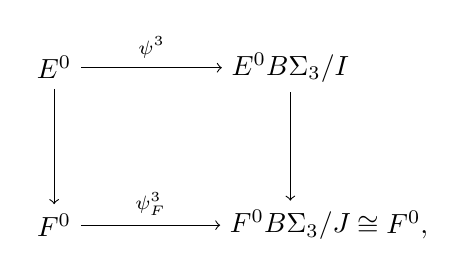
\begin{tikzpicture}
        \node (LT) at (0, 2) {$E^0$}; 
        \node (RT) at (3, 2) {$E^0 B\Sigma_3 / I$}; 
        \node (LB) at (0, 0) {$F^0$}; 
        \node (MB) at (3, 0) {$F^0 B\Sigma_3 / J$}; 
        \node (RB) at (4.3, 0) {$\cong F^0,$}; 
        \draw [->] (LT) -- node [above] {$\scriptstyle \p$} (RT); 
        \draw [->] (LT) -- (LB); 
        \draw [->] (RT) -- (MB); 
        \draw [->] (LB) -- node [above] {$\scriptstyle \psi_F^3$} (MB); 
\end{tikzpicture}
\end{center}
where $\psi_F^3$ is the $K(1)$-local power operation induced by $\p$, and $J \cong F^0 \otimes_{E^0} I$ is the transfer ideal (\cf \eqref{transfer}).  
Recall from \isog{i} and Corollary \ref{cor:psi3} that $\p$ arises from the universal degree-3 isogeny 
which is parametrized by the ring $S_3$ with 
\[
 \HS_3 = \big( S_3 \big)_{(3,h)}^\wedge \cong E^0 B\Sigma_3 / I.  
\]
The vertical maps are induced by the $K(1)$-localization $E \to F$.  In terms of 
homotopy groups, this is obtained by inverting the generator $h$ (so that 
the resulting formal group is of height at most 1) and completing at the prime 3 (\cf \cite[Corollary 1.5.5]{hovey}): 
\[
 E_* = \BZ_9 \llbracket h \rrbracket [u^{\pm1}] \qquad \ad \qquad F_* = \BZ_9 \llbracket h \rrbracket [h^{-1}]_3^\wedge [u^{\pm1}], 
\]
where 
\begin{equation}
\label{K(1)homotopy}
 F_0 = \BZ_9 (\!(h)\!)_3^\wedge = \varprojlim_k \BZ_9 (\!(h)\!) /(3^k) = 
 \left.\left\{\sum_{n = -\infty}^{\infty} c_n h^n~\right|~c_n \in \BZ_9, 
 \lim_{n \to -\infty} c_n = 0\right\}.  
\end{equation}
The formal group $\HC$ over $E^0$ has a unique order-3 subgroup after being pulled back to $F^0$ (\cf Remark \ref{rmk:dmod3}), 
and the map 
\[
 E^0 B\Sigma_3 / I \to F^0 B\Sigma_3 / J \cong F^0 
\]
classifies this subgroup.  Along the base change 
\[
 E^0 B\Sigma_3 / I \to F^0 \otimes_{E^0} (E^0 B\Sigma_3 / I) \cong (F^0 \otimes_{E^0} E^0 B\Sigma_3) / J \cong F^0 B\Sigma_3 / J, 
\]
the special fiber of the 3-divisible group of $\HC$ which consists solely of a formal component may split into formal and \'etale components.  
We want to take the formal component so as to keep track of the unique order-3 subgroup of the formal group over $F^0$.  
This subgroup gives rise to the $K(1)$-local power operation $\psi_F^3$.  

As in \isog{i}, the ring 
\[
 S_3 = S[\A] \big/ \big( w(\A) \big) 
\]
parametrizes order-3 subgroups of $C$.  Since 
\[
 w(\A) = \A^4 - 6 \A^2 + (h - 12) \A - 3 \equiv \A (\A^3 + h) \md 3, 
\]
the equation $w(\A) = 0$ has a unique root $\A = 0$ in $\BF_3 (\!(h)\!)$ (in view of \eqref{K(1)homotopy}, $\A^3 + h$ cannot be zero).  
By Hensel's lemma this unique root lifts to a root in $\BZ_9 (\!(h)\!)_3^\wedge$; 
it corresponds to the unique order-3 subgroup of $\HC$ over $F^0 = \BZ_9 (\!(h)\!)_3^\wedge$.  
Plugging this specific value of $\A$ into the formulas of $\p$ in Corollary \ref{cor:psi3}, we then get an endomorphism of the ring $F^0$.  
This endomorphism is the $K(1)$-local power operation $\psi_F^3$.  

Explicitly, with $h$ invertible in $F^0$, we can solve for $\A$ from the equation $w(\A) = 0$ by first writing 
\[
 \A = (3 + 6 \A^2 - \A^4) / (h - 12) = (3 + 6 \A^2 - \A^4) \cdot \sum_{n = 1}^\infty 12^{n-1} h^{-n} 
\]
and then substituting $\A$ recursively.  We then plug this into $\p(h)$ and get 
\[
 \psi_F^3(h) = h^3 - 36 h^2 + 372 h - 996 + 186 h^{-1} + 2232 h^{-2} + \text{lower degree terms}.  
\]
Similarly, writing $h$ as $a^2 + 4$ in $w(\A) = 0$, we solve for $\A$ in terms of $a$ and get 
\[
 \psi_F^3(a) = a^3 - 12 a - 6 a^{-1} - 84 a^{-3} - 933 a^{-5} - 10956 a^{-7} + \text{lower degree terms}.  
\]


\appendix
\section{Appendix}

Here we list long formulas whose appearance in the main body might affect readability.  
The calculations involve power series expansions and basic manipulations of long polynomials with large coefficients 
(division, factorization, and finding greatest common divisors).  
They are done using the software {\em Wolfram Mathematica 8}.  
The commands \texttt{Reduce} and \texttt{Solve} are used to extract relations out of given identities.  


\subsection{Formulas in the proof of Proposition \ref{prop:tors}}
\label{apx:tors}

\begin{equation*}
\begin{split}
 \Tf(u) = & - \frac{u^4}{a^2} \big( u^8 + 3 a u^7 + 3 a^2 u^6 + (a^3 + 7 a) u^5 + (6 a^2 - 6) u^4 + 9 a u^3 + (-a^2 \\
          & + 8) u^2 - 3 a u - 3 \big), \\
 Q_1(v) = & ~ a v^2 + (d^2 + 2 a d - 1) v + \frac{d^4}{a} + 2 d^3 + a d^2 - \frac{2 d^2}{a} - d + \frac{1}{a}, \\
 R_1(v) = & ~ (\frac{d^6}{a} + 2 d^5 + a d^4 - \frac{3 d^4}{a} + 2 d^3 + \frac{3 d^2}{a} - \frac{1}{a}) v + \frac{d^7}{a} + 2 d^6 + a d^5 - \frac{2 d^5}{a} \qquad \qquad \\
          & + 2 d^4 + \frac{d^3}{a}, 
\end{split}
\end{equation*}
\begin{equation*}
\begin{split}
 Q_2(v) = & ~ \frac{a}{(d^6 + 2 a d^5 + a^2 d^4 - 3 d^4 + 2 a d^3 + 3 d^2 - 1)^2} \big( (a d^6 + 2 a^2 d^5 + a^3 d^4 - 3 a d^4 \\
          & + 2 a^2 d^3 + 3 a d^2 - a) v - d^8 - 2 a d^7 - a^2 d^6 + 4 d^6 - a d^5 + a^2 d^4 - 6 d^4 \\
          & + 4 a d^3 + 4 d^2 - a d - 1 \big), \\
 R_2 = & - \frac{a d^4}{(d^6 + 2 a d^5 + a^2 d^4 - 3 d^4 + 2 a d^3 + 3 d^2 - 1)^2} (d^8 + 3 a d^7 + 3 a^2 d^6 + a^3 d^5 \\
       & + 7 a d^5 + 6 a^2 d^4 - 6 d^4 + 9 a d^3 - a^2 d^2 + 8 d^2 - 3 a d - 3), \\
 K(u) = & ~ \frac{1}{a} \big( u^6 + 2 a u^5 + (a^2 - 3) u^4 + 2 a u^3 + 3 u^2 - 1 \big), \\
 L(u) = & ~ \frac{1}{a} \big( u^7 + 2 a u^6 + (a^2 - 2) u^5 + 2 a u^4 + u^3 \big), \\
 M(u) = & ~ \frac{1}{a^2 (a + 4)^2 (a - 4)^2} \big( (10 a^3 - 112 a) u^5 + (19 a^4 - 217 a^2 - 16) u^4 + (8 a^5 \\
        & - 126 a^3 + 304 a) u^3 + (-a^6 + 34 a^4 - 266 a^2 + 32) u^2 + (28 a^3 - 384 a) u \\
        & - 4 a^4 + 51 a^2 - 16 \big), \\
 N(u) = & - \frac{1}{a (a + 4)^2 (a - 4)^2} \big( (10 a^3 - 112 a) u^7 + (29 a^4 - 329 a^2 - 16) u^6 + (27 a^5 \\
        & - 313 a^3 - 48 a) u^5 + (7 a^6 - 15 a^4 - 837 a^2 - 16) u^4 + (-a^7 + 66 a^5 - 714 a^3 \\
        & + 528 a) u^3 + (-4 a^6 + 137 a^4 - 1147 a^2 + 80) u^2 + (-12 a^5 + 237 a^3 \\
        & - 1200 a) u + a^6 - 44 a^4 + 409 a^2 - 48 \big).  
\end{split}
\end{equation*}


\subsection{Formulas in the proof of Proposition \ref{prop:isog}}
\label{apx:isog}

\begin{equation*}
\begin{split}
 v = & ~ u^3 - a u^4 + (a^2 + 1) u^5 + (-a^3 - 3 a) u^6 + (a^4 + 6 a^2 + 1) u^7 + (-a^5 - 10 a^3 \\
     & - 6 a) u^8 + (a^6 + 15 a^4 + 20 a^2 + 1) u^9 + \text{higher degree terms}.  
\end{split}
\end{equation*}

The group law on $C$ satisfies: 
\begin{itemize}
 \item given $P(u,v)$, the coordinates of $-P$ are 
 \[
  u_0 = -\frac{v}{u (u + v)} \qquad \ad \qquad v_0 = -\frac{v^2}{u^2 (u + v)}; 
 \]

 \item given $P_1(u_1,v_1)$ and $P_2(u_2,v_2)$, the coordinates of $-(P_1 + P_2)$ are 
 \[
  u_3 = a k - \frac{b}{1 + k} - u_1 - u_2 \qquad \ad \qquad v_3 = k u_3 + b, 
 \]
 where 
 \[
  k = \frac{v_1 - v_2}{u_1 - u_2} \qquad \ad \qquad b = \frac{u_1 v_2 - u_2 v_1}{u_1 - u_2}.  
 \]
\end{itemize}
Given $P(u,v)$ and $Q(d,e)$, with the above notations and formulas, 
\begin{itemize}
 \item set 
 \[
  (u_1,v_1) = \left( -\frac{v}{u (u + v)},-\frac{v^2}{u^2 (u + v)} \right) \qquad \ad \qquad (u_2,v_2) = (d,e), 
 \]
 so that 
 \begin{equation}
 \label{P-Q}
  P - Q = (u_3,v_3); 
 \end{equation}

 \item set 
 \[
  (u_1,v_1) = (u,v) \qquad \ad \qquad (u_2,v_2) = (d,e), 
 \]
 so that 
 \begin{equation}
 \label{P+Q}
  P + Q = \left( -\frac{v_3}{u_3 (u_3 + v_3)},-\frac{v_3^2}{u_3^2 (u_3 + v_3)} \right).  
 \end{equation}
\end{itemize}
Plugging the coordinates of $P - Q$ and $P + Q$ into \eqref{u'v'def}, and in view of \eqref{f}, 
we then have in \eqref{u'v'formula} 
\begin{equation*}
\begin{split}
 \A = & -\frac{1}{(a + 4) (a - 4)} \big( a d^7 + (3 a^2 - 2) d^6 + (3 a^3 - 6 a) d^5 + (a^4 + a^2 + 2) d^4 \\
      & + (4 a^3 - 15 a) d^3 + (a^2 + 2) d^2 - 12 a d -18 \big), \\
 \beta = & -\frac{1}{a^2 (a + 4) (a - 4)} \big( (a^3 - 11 a) d^7 + (3 a^4 - 33 a^2 - 4) d^6 + (3 a^5 - 33 a^3 \\
         & - 15 a) d^5 + (a^6 - 4 a^4 - 96 a^2 - 4) d^4 + (6 a^5 - 80 a^3 + 31 a) d^3 + (10 a^4 \\
         & - 153 a^2 + 20) d^2 + (3 a^3 - 117 a) d - 6 a^2 - 12 \big).  
\end{split}
\end{equation*}
We have the normalizing factor 
\begin{equation*}
\begin{split}
 \frac{\A^3}{\beta} = & -\frac{1}{(a + 4) (a - 4)} \big( 3 a d^7 + (9 a^2 - 4) d^6 + (9 a^3 - 13 a) d^5 + (3 a^4 + 6 a^2 + 12) d^4 \\
                      & + (11 a^3 - 15 a) d^3 + (-a^4 + 21 a^2 - 12) d^2 + (-3 a^3 + 9 a) d - 4 a^2 + 4 \big).  
\end{split}
\end{equation*}
More extended formulas for $u'$ and $v'$ in \eqref{u'v'formula} are needed to determine the coefficients in the Weierstrass equation of $C'$: 
\begin{equation*}
\begin{split}
 u' = & -\frac{1}{(a + 4) (a - 4)} \big( (a d^7 + 3 a^2 d^6 - 2 d^6 + 3 a^3 d^5 - 6 a d^5 + a^4 d^4 + a^2 d^4 + 2 d^4 \\
      & + 4 a^3 d^3 - 15 a d^3 + a^2 d^2 + 2 d^2 - 12 a d - 18) u + (-a^2 d^7 + 12 d^7 - 3 a^3 d^6 \\
      & + 36 a d^6 - 3 a^4 d^5 + 36 a^2 d^5 + 4 d^5 - a^5 d^4 + 5 a^3 d^4 + 94 a d^4 - 6 a^4 d^3 + 85 a^2 d^3 \\
      & - 76 d^3 - 9 a^3 d^2 + 136 a d^2 + 60 d + 6 a) u^2 + (a^3 d^7 - 17 a d^7 + 3 a^4 d^6 - 50 a^2 d^6 \\
      & - 8 d^6 + 3 a^5 d^5 - 48 a^3 d^5 - 27 a d^5 + a^6 d^4 - 7 a^4 d^4 - 150 a^2 d^4 - 16 d^4 + 7 a^5 d^3 \\
      & - 113 a^3 d^3 + 9 a d^3 + 16 a^4 d^2 - 258 a^2 d^2 + 56 d^2 + 15 a^3 d - 237 a d+2 a^2 \\
      & - 32) u^3 + (-a^4 d^7 + 16 a^2 d^7 + 12 d^7 - 3 a^5 d^6 + 46 a^3 d^6 + 64 a d^6 - 3 a^6 d^5 \\
      & + 42 a^4 d^5 + 121 a^2 d^5 + 4 d^5 - a^7 d^4 + 3 a^5 d^4 + 209 a^3 d^4 + 122 a d^4 - 8 a^6 d^3 \\
      & + 114 a^4 d^3 + 248 a^2 d^3 - 76 d^3 - 24 a^5 d^2 + 384 a^3 d^2 - 4 a d^2 - 33 a^4 d + 519 a^2 d \\
      & + 60 d - 18 a^3 + 282 a) u^4 + (a^5 d^7 - 9 a^3 d^7 - 117 a d^7 + 3 a^6 d^6 - 24 a^4 d^6 \\
      & - 396 a^2 d^6 - 24 d^6 + 3 a^7 d^5 - 18 a^5 d^5 - 484 a^3 d^5 - 111 a d^5 + a^8 d^4 + 7 a^6 d^4 \\
      & - 307 a^4 d^4 - 1038 a^2 d^4 + 9 a^7 d^3 - 73 a^5 d^3 - 1181 a^3 d^3 + 573 a d^3 + 33 a^6 d^2 \\
      & - 451 a^4 d^2 - 1236 a^2 d^2 + 72 d^2 + 54 a^5 d - 807 a^3 d - 873 a d + 36 a^4 - 570 a^2 \\
      & - 48) u^5 + (-a^6 d^7 - 5 a^4 d^7 + 337 a^2 d^7 + 12 d^7 - 3 a^7 d^6 - 19 a^5 d^6 + 1064 a^3 d^6 \\
      & + 204 a d^6 - 3 a^8 d^5 - 27 a^6 d^5 + 1164 a^4 d^5 + 638 a^2 d^5 + 4 d^5 - a^9 d^4 - 24 a^7 d^4 \\
      & + 441 a^5 d^4 + 3195 a^3 d^4 + 182 a d^4 - 10 a^8 d^3 - 22 a^6 d^3 + 2956 a^4 d^3 - 645 a^2 d^3 \\
      & - 76 d^3 - 43 a^7 d^2 + 403 a^5 d^2 + 4594 a^3 d^2 - 544 a d^2 - 78 a^6 d + 996 a^4 d \\
      & + 4014 a^2 d + 60 d - 57 a^5 + 852 a^3 + 942 a) u^6 + \text{higher degree terms} \big), \\
 v' = & -\frac{1}{a^2 (a + 4) (a - 4)} \big( (a^3 d^7 - 11 a d^7 + 3 a^4 d^6 - 33 a^2 d^6 - 4 d^6 + 3 a^5 d^5 - 33 a^3 d^5 \\
      & - 15 a d^5 + a^6 d^4 - 4 a^4 d^4 - 96 a^2 d^4 - 4 d^4 + 6 a^5 d^3 - 80 a^3 d^3 + 31 a d^3 + 10 a^4 d^2 \\
      & - 153 a^2 d^2 + 20 d^2 + 3 a^3 d - 117 a d - 6 a^2 - 12) u^3 + (-2 a^4 d^7 + 28 a^2 d^7 \\
      & - 6 a^5 d^6 + 82 a^3 d^6 + 28 a d^6 - 6 a^6 d^5 + 78 a^4 d^5 + 90 a^2 d^5 - 2 a^7 d^4 + 8 a^5 d^4 \\
      & + 294 a^3 d^4 + 20 a d^4 - 14 a^6 d^3 + 202 a^4 d^3 + 72 a^2 d^3 - 32 a^5 d^2 + 510 a^3 d^2 \\
      & - 124 a d^2 - 30 a^4 d + 546 a^2 d - 6 a^3 + 204 a) u^4 + (3 a^5 d^7 - 38 a^3 d^7 - 107 a d^7 \\
      & + 9 a^6 d^6 - 108 a^4 d^6 - 409 a^2 d^6 - 4 d^6 + 9 a^7 d^5 - 96 a^5 d^5 - 590 a^3 d^5 - 47 a d^5 \\
      & + 3 a^8 d^4 + a^6 d^4 - 646 a^4 d^4 - 912 a^2 d^4 - 4 d^4 + 24 a^7 d^3 - 292 a^5 d^3 - 1249 a^3 d^3 \\
      & + 639 a d^3 + 70 a^6 d^2 - 1057 a^4 d^2 - 849 a^2 d^2 + 20 d^2 + 93 a^5 d - 1512 a^3 d \\
      & - 597 a d + 48 a^4 - 870 a^2 - 12) u^5 + (-4 a^6 d^7 + 24 a^4 d^7 + 583 a^2 d^7 - 12 a^7 d^6 
\end{split}
\end{equation*}
\begin{equation*}
\begin{split}
\qquad& + 60 a^5 d^6 + 1923 a^3 d^6 + 156 a d^6 - 12 a^8 d^5 + 36 a^6 d^5 + 2268 a^4 d^5 + 639 a^2 d^5 \\
      & - 4 a^9 d^4 - 40 a^7 d^4 + 1256 a^5 d^4 + 5128 a^3 d^4 + 140 a d^4 - 36 a^8 d^3 + 229 a^6 d^3 \\
      & + 5409 a^4 d^3 - 2227 a^2 d^3 - 127 a^7 d^2 + 1597 a^5 d^2 + 6835 a^3 d^2 - 748 a d^2 \\
      & - 201 a^6 d + 2952 a^4 d + 5277 a^2 d - 129 a^5 + 2130 a^3 + 708 a) u^6 + (5 a^7 d^7 \\
      & + 35 a^5 d^7 - 1754 a^3 d^7 - 275 a d^7 + 15 a^8 d^6 + 125 a^6 d^6 - 5511 a^4 d^6 - 1833 a^2 d^6 \\
      & - 4 d^6 + 15 a^9 d^5 + 165 a^7 d^5 - 5988 a^5 d^5 - 4312 a^3 d^5 - 103 a d^5 + 5 a^{10} d^4 \\
      & + 130 a^8 d^4 - 2183 a^6 d^4 - 17022 a^4 d^4 - 2940 a^2 d^4 - 4 d^4 + 50 a^9 d^3 + 159 a^7 d^3 \\
      & - 15035 a^5 d^3 + 179 a^3 d^3 + 1703 a d^3 + 206 a^8 d^2 - 1708 a^6 d^2 - 25304 a^4 d^2 \\
      & + 1431 a^2 d^2 + 20 d^2 + 363 a^7 d - 4398 a^5 d - 23694 a^3 d - 1437 a d + 258 a^6 \\
      & - 3816 a^4 - 7026 a^2 - 12) u^7 + (-6 a^8 d^7 - 164 a^6 d^7 + 3864 a^4 d^7 + 3365 a^2 d^7 \\
      & - 18 a^9 d^6 - 522 a^7 d^6 + 11837 a^5 d^6 + 13701 a^3 d^6 + 448 a d^6 - 18 a^{10} d^5 \\
      & - 582 a^8 d^5 + 12275 a^6 d^5 + 21828 a^4 d^5 + 2395 a^2 d^5 - 6 a^{11} d^4 - 296 a^9 d^4 \\
      & + 3283 a^7 d^4 + 43960 a^5 d^4 + 30290 a^3 d^4 + 424 a d^4 - 66 a^{10} d^3 - 1099 a^8 d^3 \\
      & + 32246 a^6 d^3 + 30529 a^4 d^3 - 17045 a^2 d^3 - 310 a^9 d^2 + 679 a^7 d^2 + 66726 a^5 d^2 \\
      & + 24833 a^3 d^2 - 2192 a d^2 - 588 a^8 d + 4809 a^6 d + 73578 a^4 d + 23685 a^2 d \\
      & - 444 a^7 + 5316 a^5 + 30936 a^3 + 1704 a) u^8 + (7 a^9 d^7 + 392 a^7 d^7 - 6863 a^5 d^7 \\
      & - 17458 a^3 d^7 - 515 a d^7 + 21 a^{10} d^6 + 1218 a^8 d^6 - 20647 a^6 d^6 - 61745 a^4 d^6 \\
      & - 6709 a^2 d^6 - 4 d^6 + 21 a^{11} d^5 + 1302 a^9 d^5 - 20664 a^7 d^5 - 81924 a^5 d^5 \\
      & - 22146 a^3 d^5 - 183 a d^5 + 7 a^{12} d^4 + 567 a^{10} d^4 - 3982 a^8 d^4 - 97733 a^6 d^4 \\
      & - 158644 a^4 d^4 - 8392 a^2 d^4 - 4 d^4 + 84 a^{11} d^3 + 2878 a^9 d^3 - 57242 a^7 d^3 \\
      & - 160981 a^5 d^3 + 59447 a^3 d^3  +3223 a d^3 + 442 a^{10} d^2 + 2563 a^8 d^2 - 142138 a^6 d^2 \\
      & - 189134 a^4 d^2 + 18323 a^2 d^2 + 20 d^2 + 885 a^9 d - 2382 a^7 d - 179958 a^5 d \\
      & - 164688 a^3 d - 2637 a d + 696 a^8 - 5400 a^6 - 92938 a^4 - 29078 a^2 - 12) u^9 \\
      & + \text{higher degree terms} \big).  
\end{split}
\end{equation*}


\subsection{Formulas in Remark \ref{rmk:velu}}
\label{apx:velu}

We follow the notations in ``Isogenies of odd degree'' of \cite[Section 2.4]{kohel} 
(note that the polynomial ``$\psi(x)$'' there determines our universal degree-3 isogeny ``$\psi$'').  

Associated to the elliptic curve 
\[
 C \co y^2 + a x y + a y = x^3 + x^2, 
\]
we have 
\[
 a_1 = a, \quad a_3 = a, \quad b_2 = a^2 + 4, \quad b_4 = a^2, \quad b_6 = a^2, \quad \psi_2 = 2 y + a x + a.  
\]
Associated to the isogeny 
\[
 \psi \co C \to C', 
\]
we have 
\[
 d = 3 \qquad \ad \qquad n = 1.  
\]
Moreover, since the kernel of $\psi$ is the subgroup $G$ generated by the 3-torsion point $Q$ with $x$-coordinate $s$, 
and since $-Q$ has the same $x$-coordinate, the polynomial which defines the ideal sheaf for $G$ is then 
\[
 \psi(x) = x - s.  
\]
Thus in the identity 
\[
 \psi(x) = x^n - s_1 x^{n-1} + \cdots + (-1)^n s_n, 
\]
we have 
\[
 s_1 = s, \qquad \ad \qquad s_i = 0 \quad \text{for} \quad i > 1.  
\]
We then have 
\begin{equation*}
\begin{split}
     \phi(x) = & ~ x^3 - 2 s x^2 + (7 s^2+ a^2 s + 4 s + a^2) x - 2 s^3 + a^2 s + a^2, \\
 \omega(x,y) = & ~ \big( x^3 - 3 s x^2 + (-3 s^2 - a^2 s - 4 s - a^2) x - 3 s^3 - a^2 s^2 - 4 s^2 - 3 a^2 s - 2 a^2 \big) y \\
               & + (-6 a s^2 - a^3 s - 4 a s - a^3) x^2 + (3 a s^3 - 3 a s^2 -2 a^3 s - 2 a s - 2 a^3) x \\
               & - a s^4 - a s^3 - 2 a s^2 - a^3 s - a^3.  
\end{split}
\end{equation*}
In view of \eqref{Tw}, the 4-torsion point $(0,0)$ on $C$ then maps to 
\[
 (x_0, y_0) \coloneqq \left( \frac{\phi(0)}{\psi(0)^2}, \frac{\omega(0,0)}{\psi(0)^3} \right), 
\]
where 
\begin{equation}
\label{x_0y_0}
\begin{split}
 x_0 = & ~ 6 s^3 + (2 a^2 + 5) s^2 + (5 a^2 - 6) s + 3 a^2, \\
 y_0 = & ~ (- 9 a - 6 a^{-1}) s^3 + (-3 a^3 - 8 a - 8 a^{-1}) s^2 - 7 a^3 s - 4 a^3 - 9 a.  
\end{split}
\end{equation}

The equation of $C'$ is given by 
\[
 y^2 + a x y + a y = x^3 + x^2 - 5 t x - (a^2 + 4) t - 7 w, 
\]
where 
\[
 t = 6 s^2 + (a^2 + 4) s + a^2 \quad \ad \quad w = 10 s^3 + (2 a^2 + 8) s^2 + 3 a^2 s + a^2.  
\]
We normalize this equation into the form of \eqref{Cxy} by making a sequence of changes of variables, where $x'$ and $y'$ are the variables after each change: 
\begin{itemize}
 \item set 
 \[
  ~x = x' + x_0 \qquad \ad \qquad y = y' + y_0,~ 
 \]
 where $x_0$ and $y_0$ are given in \eqref{x_0y_0}; 

 \item set 
 \[
  \qquad x = x' \qquad \ad \qquad y = y' + k x, 
 \]
 where 
 \[
  k = -6 a^{-1} s^3 + (-2 a - 8 a^{-1}) s^2 - 6 a s - 5 a; 
 \]

 \item set 
 \[
  x = \lambda^{-2} x' \qquad \ad \qquad y = \lambda^{-3} y', 
 \]
 where 
 \[
  \lambda = s + 1.  
 \]
\end{itemize}

For the congruence \eqref{tmod3}, in view of \eqref{g} and \eqref{f}, we have 
\begin{equation*}
\begin{split}
 s^{-1} = & ~ e / d \\
        = & ~ g(d) / d \\
        = & ~ \frac{1}{a (a + 4) (a - 4)} \big( 6 d^7 + 17 a d^6 + (15 a^2 + 2) d^5 + (3 a^3 + 48 a) d^4 \\
          & + (-a^4 + 35 a^2 - 38) d^3 + (-4 a^3 + 69 a) d^2 + (-6 a^2 + 30) d - 6 a \big).  
\end{split}
\end{equation*}
The congruence then follows from Remark \ref{rmk:dmod3}.  


%\nocite{*}
%\bibliographystyle{amsalpha}
%\bibliography{p3}
%\end{document}

\renewcommand\refname{Bibliography}

\newcommand{\MRn}[2]{\href{http://www.ams.org/mathscinet-getitem?mr=#1}{MR#1 #2}}
\begin{thebibliography}

\bibitem[AHS01]{cube}
M.~Ando, M.~J. Hopkins, and N.~P. Strickland, \emph{Elliptic spectra, the
  {W}itten genus and the theorem of the cube}, Invent. Math. \textbf{146}
  (2001), no.~3, 595--687. \MRn{1869850}{(2002g:55009)}

\bibitem[BGJGP05]{poonen}
Matthew~H. Baker, Enrique Gonz{\'a}lez-Jim{\'e}nez, Josep Gonz{\'a}lez, and
  Bjorn Poonen, \emph{Finiteness results for modular curves of genus at least
  2}, Amer. J. Math. \textbf{127} (2005), no.~6, 1325--1387. \MRn{2183527}{(2006i:11065)}

\bibitem[BMMS86]{H_infty}
R.~R. Bruner, J.~P. May, J.~E. McClure, and M.~Steinberger, \emph{{$H\sb \infty
  $} ring spectra and their applications}, Lecture Notes in Mathematics, vol.
  1176, Springer-Verlag, Berlin, 1986. \MRn{836132}{(88e:55001)}

\bibitem[BW05]{BW}
James Borger and Ben Wieland, \emph{Plethystic algebra}, Adv. Math.
  \textbf{194} (2005), no.~2, 246--283. \MRn{2139914}{(2006i:13044)}

\bibitem[EKMM97]{EKMM}
A.~D. Elmendorf, I.~Kriz, M.~A. Mandell, and J.~P. May, \emph{Rings, modules,
  and algebras in stable homotopy theory}, Mathematical Surveys and Monographs,
  vol.~47, American Mathematical Society, Providence, RI, 1997, With an
  appendix by M. Cole. \MRn{1417719}{(97h:55006)}

\bibitem[Gre88]{blind}
J.~P.~C. Greenlees, \emph{How blind is your favourite cohomology theory?},
  Exposition. Math. \textbf{6} (1988), no.~3, 193--208. \MRn{949783}{(89j:55001)}

\bibitem[GW10]{GW}
Ulrich G{\"o}rtz and Torsten Wedhorn, \emph{Algebraic geometry {I}}, Advanced
  Lectures in Mathematics, Vieweg + Teubner, Wiesbaden, 2010, Schemes with
  examples and exercises. \MRn{2675155}{(2011f:14001)}

\bibitem[Hop]{K(1)E_infty}
M.~J. Hopkins, \emph{K(1)-local ${E}_\infty$ ring spectra}, available at
  \url{http://www.math.rochester.edu/u/faculty/doug/otherpapers/knlocal.pdf}.

\bibitem[Hov97]{hovey}
Mark~A. Hovey, \emph{{$v\sb n$}-elements in ring spectra and applications to
  bordism theory}, Duke Math. J. \textbf{88} (1997), no.~2, 327--356.
  \MRn{1455523}{(98d:55017)}

\bibitem[Hus04]{ec}
Dale Husem{\"o}ller, \emph{Elliptic curves}, second ed., Graduate Texts in
  Mathematics, vol. 111, Springer-Verlag, New York, 2004, With appendices by
  Otto Forster, Ruth Lawrence and Stefan Theisen. \MRn{2024529}{(2005a:11078)}

\bibitem[KM85]{KM}
Nicholas~M. Katz and Barry Mazur, \emph{Arithmetic moduli of elliptic curves},
  Annals of Mathematics Studies, vol. 108, Princeton University Press,
  Princeton, NJ, 1985. \MRn{772569}{(86i:11024)}

\bibitem[Koh96]{kohel}
David Kohel, \emph{Endomorphism rings of elliptic curves over finite fields},
  Ph.D. thesis, University of California, Berkeley, 1996,
  available at \url{http://echidna.maths.usyd.edu.au/kohel/pub/thesis.pdf}.

\bibitem[MFK94]{GIT}
D.~Mumford, J.~Fogarty, and F.~Kirwan, \emph{Geometric invariant theory}, third
  ed., Ergebnisse der Mathematik und ihrer Grenzgebiete (2) [Results in
  Mathematics and Related Areas (2)], vol.~34, Springer-Verlag, Berlin, 1994.
  \MRn{1304906}{(95m:14012)}

\bibitem[MR09]{tmf3}
Mark Mahowald and Charles Rezk, \emph{Topological modular forms of level 3},
  Pure Appl. Math. Q. \textbf{5} (2009), no.~2, Special Issue: In honor of
  Friedrich Hirzebruch. Part 1, 853--872. \MRn{2508904}{(2010g:55010)}

\bibitem[Reza]{lpo}
Charles Rezk, \emph{Lectures on power operations},
  available at \url{http://www.math.uiuc.edu/~rezk/power-operation-lectures.dvi}.

\bibitem[Rezb]{h2p2}
\bysame, \emph{Power operations for {M}orava ${E}$-theory of height 2 at the
  prime 2}, \href{http://arxiv.org/abs/0812.1320}{arXiv:0812.1320}.

\bibitem[Rez09]{cong}
\bysame, \emph{The congruence criterion for power operations in {M}orava
  {$E$}-theory}, Homology, Homotopy Appl. \textbf{11} (2009), no.~2, 327--379.
  \MRn{2591924}{(2011e:55021)}

\bibitem[Sil09]{AEC}
Joseph~H. Silverman, \emph{The arithmetic of elliptic curves}, second ed.,
  Graduate Texts in Mathematics, vol. 106, Springer, Dordrecht, 2009.
  \MRn{2514094}{(2010i:11005)}

\bibitem[{Sta}]{stacks-project}
The {Stacks Project Authors}, \emph{{\itshape Stacks Project}},
  \url{http://math.columbia.edu/algebraic_geometry/stacks-git}.

\bibitem[Ste62]{steenrod}
N.~E. Steenrod, \emph{Cohomology operations}, Lectures by N. E. Steenrod
  written and revised by D. B. A. Epstein. Annals of Mathematics Studies, No.
  50, Princeton University Press, Princeton, N.J., 1962. \MRn{0145525}{(26
  \#3056)}

\bibitem[Str98]{Str98}
N.~P. Strickland, \emph{Morava {$E$}-theory of symmetric groups}, Topology
  \textbf{37} (1998), no.~4, 757--779. \MRn{1607736}{(99e:55008)}

\bibitem[V{\'e}l71]{velu}
Jacques V{\'e}lu, \emph{Isog\'enies entre courbes elliptiques}, C. R. Acad.
  Sci. Paris S\'er. A-B \textbf{273} (1971), A238--A241. \MRn{0294345}{(45
  \#3414)}

\bibitem[Voe03]{V}
Vladimir Voevodsky, \emph{Reduced power operations in motivic cohomology},
  Publ. Math. Inst. Hautes \'Etudes Sci. (2003), no.~98, 1--57. \MRn{2031198}{(2005b:14038a)}

\end{thebibliography}
\end{document}